% !TeX program = xelatex
% !TeX encoding = utf8
% Bài trình bày 30 phút; nguồn nội dung và nhịp nói xem README.md.
\documentclass[aspectratio=43,11pt]{beamer}
\usetheme{Madrid}
\usecolortheme{default}
\setbeamertemplate{navigation symbols}{}
\setbeamertemplate{itemize items}[circle]
\setbeamertemplate{headline}{%
  \leavevmode%
  \begin{beamercolorbox}[wd=0.55\paperwidth,ht=2.5ex,dp=1ex,leftskip=0.35cm]{section in head/foot}%
    \scriptsize\thesection.\arabic{subsection}.\hspace{0.35em}\insertsubsectionhead
  \end{beamercolorbox}%
  \begin{beamercolorbox}[wd=0.45\paperwidth,ht=2.5ex,dp=1ex]{subsection in head/foot}\hfill\end{beamercolorbox}%
}
\setbeamertemplate{frametitle}{%
  \nointerlineskip%
  \begin{beamercolorbox}[wd=\paperwidth,ht=1.05cm,dp=0.18cm,leftskip=0.35cm,rightskip=0.3cm]{frametitle}%
    \usebeamerfont{frametitle}\insertframetitle\hfill%
    \raisebox{-0.12cm}{
\includegraphics[width=1.05cm]{../assets/tdtu-logo.jpg}}%
  \end{beamercolorbox}%
}
\setbeamertemplate{footline}{%
  \leavevmode%
  \begin{beamercolorbox}[wd=0.31\paperwidth,ht=2.5ex,dp=1ex,center]{author in head/foot}%
    \tiny THỐNG KÊ TÍNH TOÁN
  \end{beamercolorbox}%
  \begin{beamercolorbox}[wd=0.29\paperwidth,ht=2.5ex,dp=1ex,center]{title in head/foot}%
    \tiny C03107 -- Bootstrap
  \end{beamercolorbox}%
  \begin{beamercolorbox}[wd=0.26\paperwidth,ht=2.5ex,dp=1ex,center]{date in head/foot}%
    \tiny Ngày trình bày
  \end{beamercolorbox}%
  \begin{beamercolorbox}[wd=0.14\paperwidth,ht=2.5ex,dp=1ex,center]{section in head/foot}%
    \tiny\insertframenumber/\inserttotalframenumber
  \end{beamercolorbox}%
}
\setbeamercolor{author in head/foot}{fg=white,bg=TDTUBlue}
\setbeamercolor{title in head/foot}{fg=white,bg=TDTUBlue!85}
\setbeamercolor{date in head/foot}{fg=white,bg=TDTUBlue!70}
\setbeamercolor{section in head/foot}{fg=white,bg=TDTUBlue}
\setbeamercolor{subsection in head/foot}{fg=white,bg=TDTUBlue!35}
\usepackage{fontspec}
\usepackage{polyglossia}
\setdefaultlanguage{vietnamese}
\setmainfont{Arial}[Path=../assets/fonts/,Extension=.ttf,UprightFont=*-Regular,BoldFont=*-Bold,ItalicFont=*-Italic,BoldItalicFont=*-BoldItalic]
\setsansfont{Arial}[Path=../assets/fonts/,Extension=.ttf,UprightFont=*-Regular,BoldFont=*-Bold,ItalicFont=*-Italic,BoldItalicFont=*-BoldItalic]
\setmonofont{NotoSansMono}[Path=../assets/fonts/,Extension=.ttf,UprightFont=*-Regular,BoldFont=*-Bold]
\usepackage{graphicx}
\usepackage{booktabs}
\definecolor{TDTUBlue}{RGB}{58,56,176}
\setbeamercolor{structure}{fg=TDTUBlue}
\setbeamercolor{title}{fg=TDTUBlue}
\setbeamercolor{frametitle}{fg=TDTUBlue,bg=white}
\setbeamercolor{palette primary}{fg=white,bg=TDTUBlue}
\setbeamercolor{palette secondary}{fg=white,bg=TDTUBlue!85}
\setbeamercolor{palette tertiary}{fg=white,bg=TDTUBlue!70}
\setbeamercolor{palette quaternary}{fg=white,bg=TDTUBlue}

\title[Khoảng tin cậy Bootstrap]{Khoảng tin cậy Bootstrap chuẩn tắc và Bootstrap cơ bản}
\subtitle{Cơ sở lý thuyết, phương pháp xây dựng và đánh giá hiệu năng}
\author[Nhóm D]{Nhóm D}
\institute{Thống kê tính toán -- C03107\\Trường Đại học Tôn Đức Thắng}
\date{}
\begin{document}
% Frame 01. Source: Bìa. Goal: Giới thiệu học phần, đề tài và nhóm. Asset: ../assets/tdtu-logo.jpg.
\begin{frame}[plain]
\centering

\includegraphics[height=1.25cm]{../assets/tdtu-logo.jpg}\par\vspace{0.15cm}
{\small TỔNG LIÊN ĐOÀN LAO ĐỘNG VIỆT NAM\par}
{\small\bfseries TRƯỜNG ĐẠI HỌC TÔN ĐỨC THẮNG -- KHOA TOÁN -- THỐNG KÊ\par}\vspace{0.25cm}
{\usebeamerfont{title}\usebeamercolor[fg]{title}\inserttitle\par}
{\small\insertsubtitle\par}\vspace{0.25cm}
{\small Môn học: Thống kê tính toán -- C03107; Học kỳ 1/2026--2027\par}
{\small Giảng viên: ThS. Bùi Thùy Trang\par}
{\small\bfseries Nhóm D\par}
\end{frame}
\section{Giới thiệu tổng quan}
\subsection{Lộ trình trình bày}
% Frame 02. Source: Tổng quan. Goal: Nêu mạch trình bày. Asset: none.
\begin{frame}[label=frame:02]{Lộ trình trình bày}
    \begin{enumerate}
        \item Bối cảnh và mục tiêu khảo sát
        \item ECDF, nguyên lý plug-in và lấy mẫu Bootstrap
        \item Cách xây dựng Normal CI và Basic CI
        \item Hai ví dụ liệt kê chính xác
        \item Mô phỏng Monte Carlo và cách đọc kết quả
        \item Ứng dụng y sinh, Percentile CI và BCa
        \item Kết luận và khuyến nghị
    \end{enumerate}
\end{frame}
\subsection{Thành viên nhóm D}
% Frame 03. Source: Bìa. Goal: Giới thiệu thành viên nhóm.
\begin{frame}{Thành viên nhóm D}
    \centering
    \renewcommand{\arraystretch}{1.45}
    \begin{tabular}{ll}
        \toprule
        Mã sinh viên & Họ và tên\\
        \midrule
        C2400121 & Phan Trí Thịnh\\
        C2400115 & Ngô Cẩm Quí\\
        C2400203 & Nguyễn Văn Kiệt\\
        C2400199 & Trần Quốc Khang\\
        \bottomrule
    \end{tabular}
\end{frame}
\subsection{Vì sao cần khoảng tin cậy Bootstrap?}
% Frame 04. Source: Phần 1. Goal: Động lực và bối cảnh. Asset: none.
\begin{frame}[label=frame:03]{Vì sao cần khoảng tin cậy Bootstrap?}
\begin{itemize}
    \item Ước lượng điểm $\hat\theta$ cho một giá trị; khoảng tin cậy cho biết độ bất định của ước lượng.
    \item Sai số chuẩn có thể khó tính; xấp xỉ chuẩn có thể kém khi mẫu nhỏ hoặc phân phối của thống kê lệch.
    \item Bootstrap dùng mẫu quan sát để xấp xỉ phân phối lấy mẫu của thống kê.
\end{itemize}
\end{frame}
\subsection{Mục tiêu và phạm vi khảo sát}
% Frame 05. Source: Phần 1. Goal: Mục tiêu, phạm vi, giới hạn. Asset: none.
\begin{frame}[label=frame:04]{Mục tiêu và phạm vi khảo sát}
\begin{itemize}
    \item Xây dựng và so sánh Normal CI và Basic CI ở mức $95\%$.
    \item Với trung bình mẫu: giải thích vị trí hai cận bằng hai ví dụ liệt kê chính xác.
    \item Đánh giá độ bao phủ và độ dài khoảng bằng mô phỏng R; dùng Percentile làm đối chiếu.
    \item BCa và các ứng dụng y sinh minh họa phạm vi mở rộng.
\end{itemize}
\end{frame}
\section{ECDF và Monte Carlo}
\subsection{Phân phối thực nghiệm ECDF}
% Frame 06. Source: Phần 2. Goal: Định nghĩa và vai trò. Asset: none.
\begin{frame}[label=frame:05]{Phân phối thực nghiệm ECDF}
Từ mẫu $x_1,\ldots,x_n$, hàm phân phối thực nghiệm là
\[
    F_n(t)=\frac1n\sum_{i=1}^n I(x_i\le t).
\]
\begin{itemize}
    \item $I$ là hàm chỉ báo: $I(x_i\le t)=1$ nếu $x_i\le t$, bằng $0$ nếu $x_i>t$.
    \item $F_n(t)$ là tỷ lệ quan sát không vượt quá $t$.
    \item Mỗi vị trí trong mẫu có khối xác suất $1/n$; giá trị lặp được cộng khối xác suất.
    \item Rút từ $F_n$ tương đương lấy mẫu có hoàn lại từ dữ liệu gốc.
\end{itemize}
\end{frame}
\subsection{Nguyên lý Plug-in}
% Frame 07. Source: Phần 2. Goal: Xấp xỉ tổng thể bằng ECDF. Asset: none.
\begin{frame}[label=frame:06]{Nguyên lý Plug-in}
Đặt $\theta=T(F)$ và $\hat\theta=T(F_n)$.
\begin{itemize}
    \item Ta không biết $F$, nên dùng $F_n$ làm tổng thể thay thế.
    \item Trên mẫu rút từ $F_n$, tính $\hat\theta^*=T(F_n^*)$.
    \item Dùng phân phối có điều kiện của $\hat\theta^*-\hat\theta$ để xấp xỉ phân phối của $\hat\theta-\theta$.
\end{itemize}
\end{frame}
\subsection{Quy trình lấy mẫu Bootstrap}
% Frame 08. Source: Phần 2. Goal: Lấy mẫu lại và tính thống kê. Asset: none.
\begin{frame}[label=frame:07]{Quy trình lấy mẫu Bootstrap}
    \small
    1. Mẫu gốc. Có $n=3$ quan sát $(1,2,3)$, với trung bình
    $\hat\theta=(1+2+3)/3=2$.

    \medskip
    2. Rút lại 3 lần cho mỗi bản sao. Sau mỗi lượt, trả quan sát
    về mẫu gốc. Cả ba giá trị $1,2,3$ đều có thể xuất hiện ở lượt kế tiếp.
    \begin{center}
        \renewcommand{\arraystretch}{1.25}
        \setlength{\tabcolsep}{5pt}
        \begin{tabular}{lcccl}
            \toprule
            Bản sao & Lượt 1 & Lượt 2 & Lượt 3 & Trung bình $\hat\theta^{*(b)}$\\
            \midrule
            $b=1$ & $\alert{1}$ & $\alert{1}$ & $3$ & $(1+1+3)/3=5/3$\\
            $b=2$ & $2$ & $3$ & $2$ & $(2+3+2)/3=7/3$\\
            $b=3$ & $3$ & $3$ & $3$ & $(3+3+3)/3=3$\\
            \bottomrule
        \end{tabular}
    \end{center}
    3. Lặp đến đủ $B$ bản sao. Tính độ lệch chuẩn hoặc các phân vị
    từ dãy trung bình Bootstrap để dựng khoảng tin cậy.
\end{frame}
\subsection{B khác K: hai nguồn biến thiên Monte Carlo}
% Frame 09. Source: Phần 2 và 6. Goal: Phân biệt số bản sao Bootstrap và số lần mô phỏng. Asset: ../assets/simulate-results/run-info.txt.
\begin{frame}[label=frame:08]{B khác K: hai nguồn biến thiên Monte Carlo}
\begin{description}
    \item[$B=1\,999$] Số mẫu Bootstrap trên \emph{mỗi} bộ dữ liệu. Chi phối độ ổn định của sai số chuẩn và phân vị ước lượng.
    \item[$K=10\,000$] Số bộ dữ liệu độc lập sinh từ tổng thể đã biết \emph{trong mỗi kịch bản}. Chi phối độ chính xác khi ước lượng coverage.
\end{description}
\medskip
Tăng $B$ giúp tính cận ổn định hơn. Tăng $K$ giúp đo hiệu năng chính xác hơn.
\end{frame}
\section{Xây dựng Normal và Basic CI}
\subsection{Normal CI: ý tưởng và công thức}
% Frame 10. Source: Phần 3. Goal: Giả định và khoảng đối xứng. Asset: none.
\begin{frame}[label=frame:09]{Normal CI: ý tưởng và công thức}
    \small
    Ước lượng sai số chuẩn bằng độ lệch chuẩn của $B$ bản sao $\hat\theta^*$, ký hiệu $\widehat{se}^{*}$. Nếu sai số có độ chệch nhỏ và xấp xỉ chuẩn, đặt
    \[
        Z=\frac{\hat\theta-\theta}{\widehat{se}^{*}}\approx N(0,1).
    \]
    Với $z=z_{1-\alpha/2}$, hai đuôi chuẩn có xác suất $\alpha/2$ mỗi bên.
    \[
    \begin{aligned}
        -z\le Z\le z
        &\iff -z\widehat{se}^{*}\le\hat\theta-\theta\le z\widehat{se}^{*}\\
        &\iff \hat\theta-z\widehat{se}^{*}\le\theta\le\hat\theta+z\widehat{se}^{*}.
    \end{aligned}
    \]
    Hai biểu thức cuối là cận của Normal CI. Ở mức $95\%$, $z\approx1.96$.
\end{frame}
\subsection{Basic CI và phép đảo phân vị}
% Frame 11. Source: Phần 3. Goal: Phản chiếu phân vị quanh ước lượng gốc. Asset: none.
\begin{frame}[label=frame:10]{Basic CI và phép đảo phân vị}
    \small
    Gọi $q_L^*,q_U^*$ là hai phân vị đuôi của $\hat\theta^*$. Theo nguyên lý plug-in, dùng các phân vị của $\hat\theta^*-\hat\theta$, tức $d_L=q_L^*-\hat\theta$ và $d_U=q_U^*-\hat\theta$, để xấp xỉ phân vị của $\hat\theta-\theta$.
    \[
        \Pr\!\left(d_L\le\hat\theta-\theta\le d_U\right)\approx 1-\alpha.
    \]
    Giải bất đẳng thức trong xác suất theo $\theta$:
    \[
    \begin{aligned}
        d_L\le\hat\theta-\theta\le d_U
        &\iff \hat\theta-d_U\le\theta\le\hat\theta-d_L\\
        &\iff 2\hat\theta-q_U^*\le\theta\le 2\hat\theta-q_L^*.
    \end{aligned}
    \]
    Vì nhân với $-1$ làm đảo chiều bất đẳng thức, phân vị trên tạo cận dưới.
\end{frame}
\section{So sánh Normal và Basic CI}
\subsection{Normal CI và Basic CI khác nhau thế nào?}
% Frame 12. Source: Phần 4. Goal: So sánh giả định và giới hạn. Asset: none.
\begin{frame}[label=frame:11]{Normal CI và Basic CI khác nhau thế nào?}
\begin{description}
    \item[Normal] Dùng sai số chuẩn và phân vị chuẩn; hai cận cách đều $\hat\theta$.
    \item[Basic] Dùng hai phân vị thực nghiệm; khoảng có thể bất đối xứng và phản chiếu hướng lệch.
\end{description}
\medskip
Cả hai có thể cho cận ngoài miền tham số. Việc dùng phân vị trong Basic không bảo đảm coverage tốt hơn.
\end{frame}
\section{Ví dụ Bootstrap}
\subsection{Ví dụ mẫu đối xứng}
% Frame 13. Source: Phần 5. Goal: Liệt kê chính xác phân phối Bootstrap. Asset: ../assets/simulate-results/example-bootstrap-distributions.pdf.
\begin{frame}[label=frame:12]{Ví dụ mẫu đối xứng}
    \small
    Mẫu gốc $(1,2,3)$ có trung bình $\hat\theta=2$. Mỗi lần rút có 3 lựa chọn, nên 3 lần rút có hoàn lại cho $3^3=27$ bộ có thứ tự.
    Chẳng hạn, $(1,1,3)$ cho $\hat\theta^*=5/3$.
    \begin{center}
        \begin{tabular}{lrrrrrrr}
            \toprule
            $\hat\theta^*$ & $1$ & $4/3$ & $5/3$ & $2$ & $7/3$ & $8/3$ & $3$\\
            Số bộ & 1 & 3 & 6 & 7 & 6 & 3 & 1\\
            \bottomrule
        \end{tabular}
    \end{center}
    Với phân vị type~1, lấy giá trị ở hạng $\lceil 27p\rceil$ sau khi sắp tăng dần. Hai hạng $1$ và $27$ cho $q_L^*=1$, $q_U^*=3$.
    \[
        CI_{\mathrm{Basic}}=[2\cdot2-3,\;2\cdot2-1]=[1,3].
    \]
\end{frame}
\subsection{Ví dụ mẫu lệch phải}
% Frame 14. Source: Phần 5. Goal: Đối chiếu cách đặt cận; số liệu theo báo cáo. Asset: ../assets/simulate-results/example-confidence-intervals.csv.
\begin{frame}[label=frame:13]{Ví dụ mẫu lệch phải}
    \small
    Mẫu $(1,1,1,9)$ có $\hat\theta=3$. Nếu rút trúng $9$ đúng $j$ lần trong 4 lượt thì $\hat\theta^*=[9j+(4-j)]/4=1+2j$.
    \begin{center}
        \begin{tabular}{lrrrrr}
            \toprule
            Số lần rút trúng $9$ & 0 & 1 & 2 & 3 & 4\\
            $\hat\theta^*$ & 1 & 3 & 5 & 7 & 9\\
            Số bộ & 81 & 108 & 54 & 12 & 1\\
            Số bộ tích lũy & 81 & 189 & 243 & 255 & 256\\
            \bottomrule
        \end{tabular}
    \end{center}
    Ví dụ, đúng một lần rút trúng $9$ có $4\cdot3^3=108$ bộ: chọn vị trí của $9$, rồi chọn một trong ba vị trí mang giá trị $1$ ở mỗi lượt còn lại.

    \medskip
    Type~1 cho hạng $\lceil256\cdot0.025\rceil=7$ và $\lceil256\cdot0.975\rceil=250$. Đọc hàng tích lũy được $q_L^*=1$, $q_U^*=7$.
\end{frame}
\subsection{Đối chiếu các khoảng trong hai ví dụ}
% Frame 15. Source: Phần 5. Goal: So sánh Normal, Basic, Percentile. Asset: ../assets/simulate-results/example-confidence-intervals.csv.
\begin{frame}[label=frame:14]{Đối chiếu các khoảng trong hai ví dụ}
    \small
    Từ bảng tần số mẫu lệch phải, mỗi nhóm có xác suất bằng số bộ chia cho $256$. Bình phương độ lệch quanh $\hat\theta=3$ rồi lấy trung bình có trọng số:
    \[
        (\widehat{se}^{*})^2=\frac{81(1-3)^2+108(3-3)^2+54(5-3)^2+12(7-3)^2+(9-3)^2}{256}=3.
    \]
    Do đó $\widehat{se}^{*}=\sqrt{3}\approx1.7321$.
    \begin{center}
        \begin{tabular}{lcc}
            \toprule
            CI $95\%$ & Mẫu đối xứng & Mẫu lệch phải\\
            \midrule
            Normal & $[1.076,\,2.924]$ & $3\pm1.96(1.7321)\approx[-0.395,\,6.395]$\\
            Basic & $[1,\,3]$ & $[6-7,\;6-1]=[-1,5]$\\
            Percentile & $[1,\,3]$ & $[1,7]$\\
            \bottomrule
        \end{tabular}
    \end{center}
    Trên mẫu lệch phải, Basic và Percentile đều dài $6$ nhưng nằm ở hai vị trí khác nhau. Phần mô phỏng sẽ đo độ bao phủ qua nhiều mẫu.
\end{frame}
\section{Mô phỏng Monte Carlo}
\subsection{Thiết kế mô phỏng Monte Carlo}
% Frame 16. Source: Phần 6. Goal: Thiết lập, seed và MCSE. Asset: ../assets/simulate-results/run-info.txt.
\begin{frame}[label=frame:15]{Thiết kế mô phỏng Monte Carlo}
\begin{itemize}
    \item Ước lượng trung bình của $N(0,1)$ ($\theta=0$) và $\operatorname{Exp}(1)$ ($\theta=1$), với $n=12,40$.
    \item Mỗi kịch bản: $K=10\,000$, $B=1\,999$, mức danh nghĩa $95\%$, phân vị R type~7.
    \item Coverage: tỷ lệ khoảng chứa $\theta$. AL: trung bình độ dài $U_k-L_k$.
    \item Sai số chuẩn Monte Carlo của coverage: $\sqrt{\widehat{CP}(1-\widehat{CP})/K}$.
\end{itemize}
\end{frame}
\subsection{Kết quả coverage}
% Frame 17. Source: Phần 6. Goal: Bốn kịch bản và mức danh nghĩa. Asset: ../assets/simulate-results/simulation-coverage.pdf; simulation-summary.csv.
\begin{frame}[label=frame:16]{Kết quả coverage}
\begin{center}
    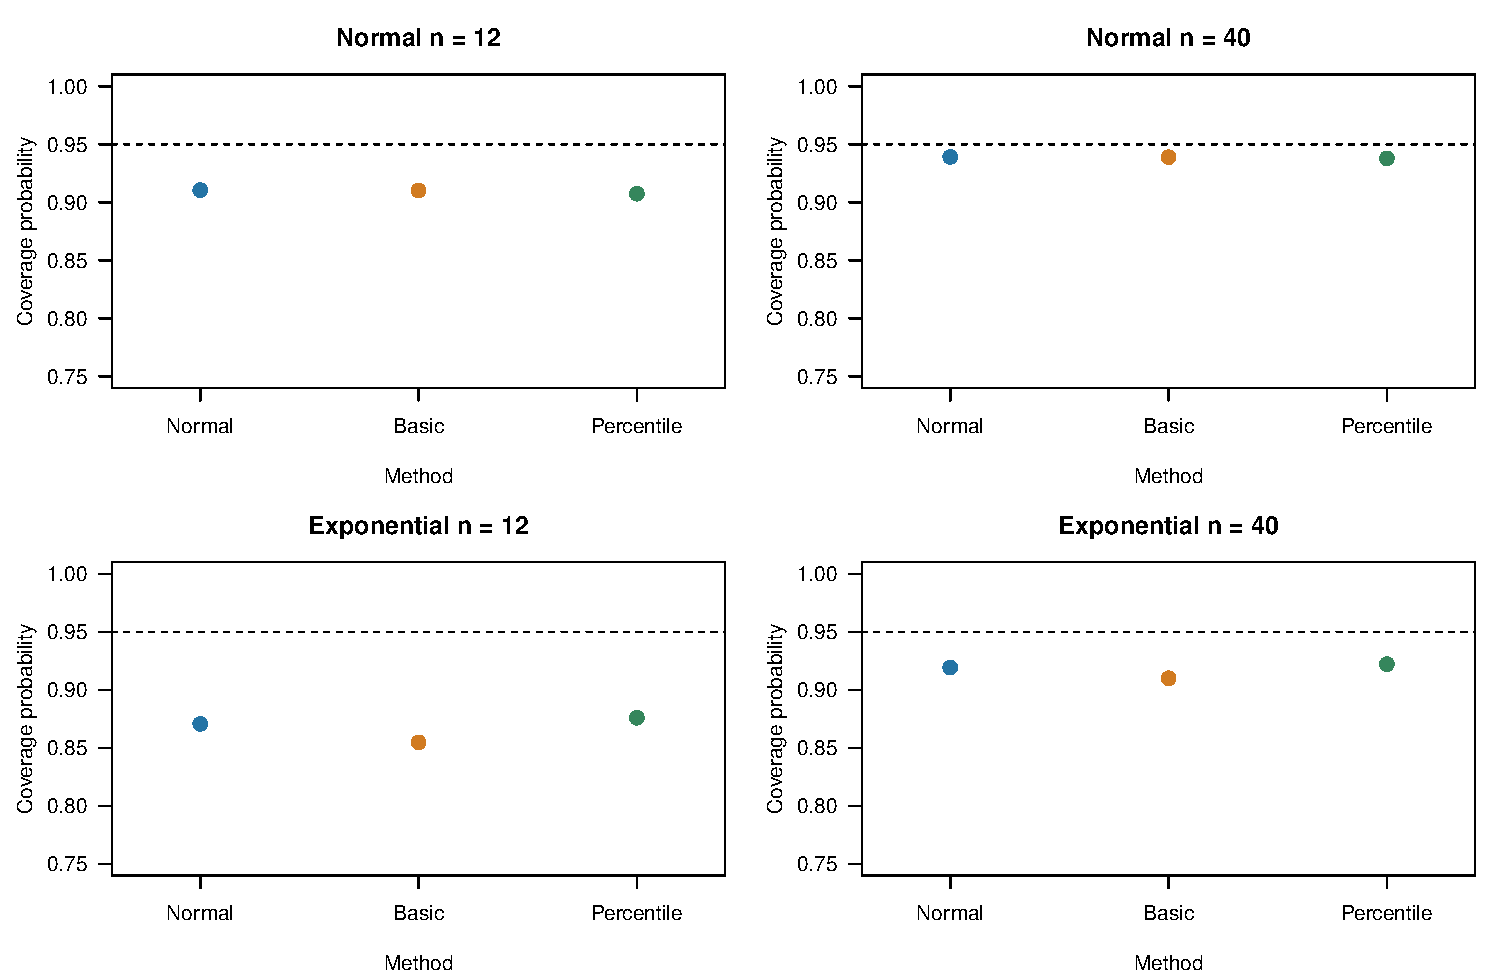
\includegraphics[width=\linewidth,height=5.4cm,keepaspectratio]{../assets/simulate-results/simulation-coverage.pdf}
\end{center}
\small Tất cả dưới $95\%$. Với $\operatorname{Exp}(1)$, $n=12$: Percentile $87.59\%$, Normal $87.06\%$, Basic $85.47\%$.
\end{frame}
\subsection{Kết quả độ dài khoảng trung bình}
% Frame 18. Source: Phần 6. Goal: Đọc AL cùng coverage. Asset: ../assets/simulate-results/simulation-average-length.pdf; simulation-summary.csv.
\begin{frame}[label=frame:17]{Kết quả độ dài khoảng trung bình}
\begin{center}
    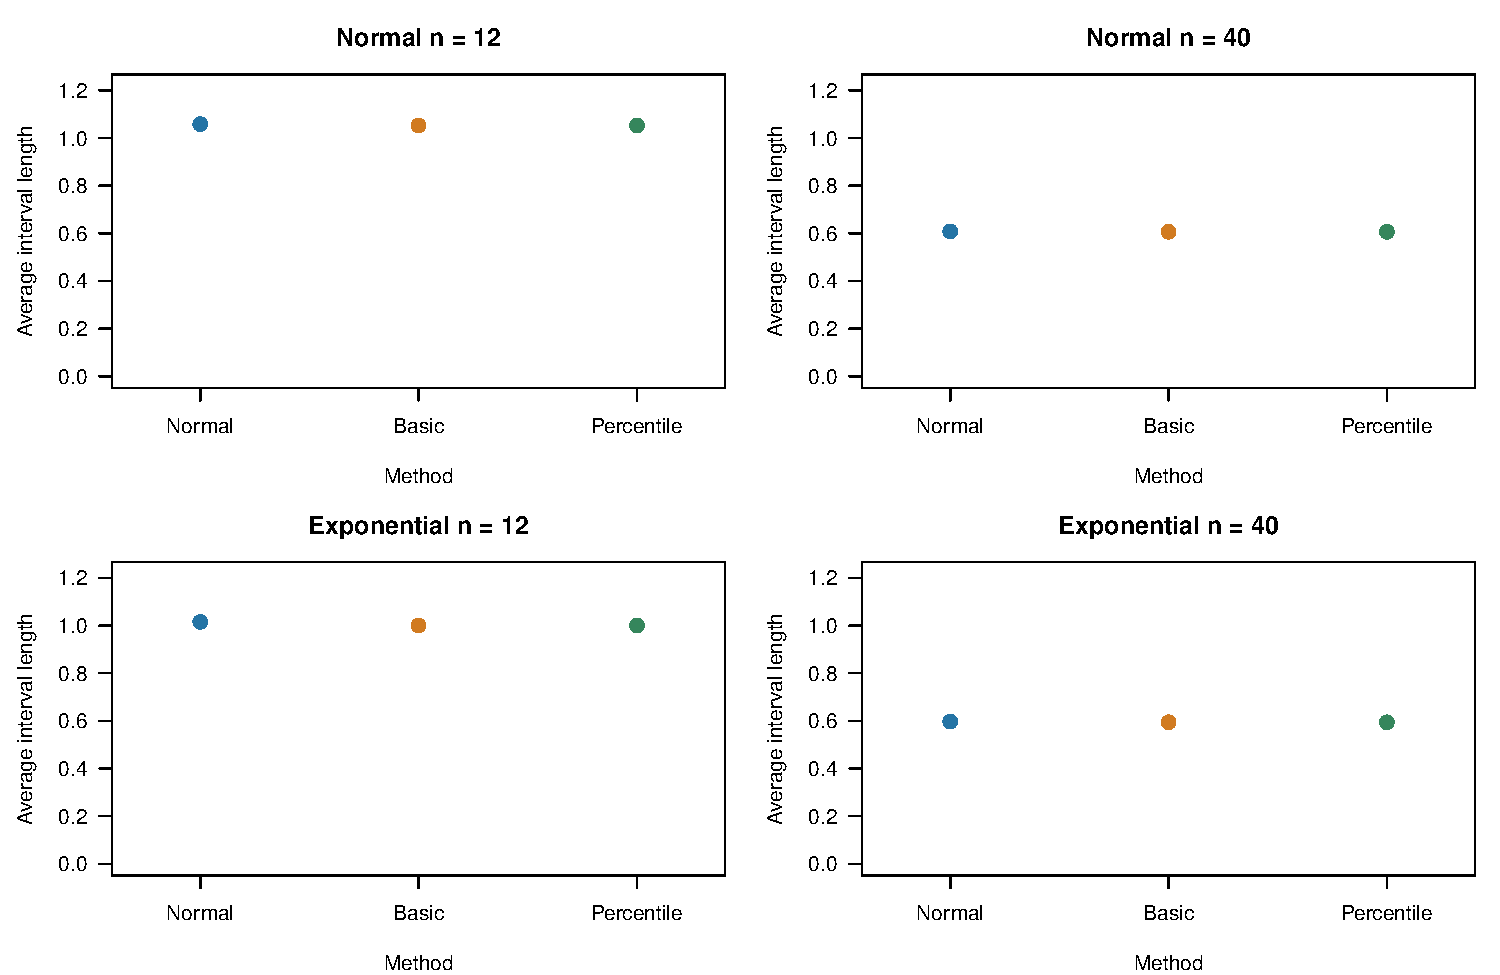
\includegraphics[width=\linewidth,height=5.4cm,keepaspectratio]{../assets/simulate-results/simulation-average-length.pdf}
\end{center}
\small Basic và Percentile có cùng độ dài $q_U^*-q_L^*$ trên từng mẫu. Normal dài hơn nhẹ trong cả bốn kịch bản.
\end{frame}
\subsection{Những điều rút ra từ mô phỏng}
% Frame 19. Source: Phần 6. Goal: Giới hạn kết luận trong thiết kế đã chạy. Asset: ../assets/simulate-results/simulation-summary.csv.
\begin{frame}[label=frame:18]{Những điều rút ra từ mô phỏng}
\begin{itemize}
    \item Từ $n=12$ lên $n=40$, coverage tăng và độ dài trung bình giảm ở cả hai tổng thể.
    \item Với tổng thể chuẩn, ba phương pháp cho coverage gần nhau. Với tổng thể mũ, Percentile cao nhất và Basic thấp nhất trong lần chạy này.
    \item Đọc coverage cùng độ dài: hai khoảng dài bằng nhau vẫn có thể bao phủ khác nhau do vị trí hai cận.
\end{itemize}
\end{frame}
\subsection{Coverage 85,47\% nghĩa là gì?}
% Frame 20. Source: Phần 6. Asset: simulation-summary.csv; run-info.txt.
\begin{frame}{Coverage 85,47\% nghĩa là gì?}
    \small
    \textbf{Kịch bản mô phỏng.} Mỗi bộ dữ liệu gồm $n=12$ quan sát từ
    $\operatorname{Exp}(1)$, với trung bình tổng thể thật $\theta=1$.
    Mỗi bộ cho một khoảng Basic CI $95\%$ từ $B=1\,999$ mẫu Bootstrap.
    \begin{center}
        \renewcommand{\arraystretch}{1.25}
        \begin{tabular}{lr}
            \toprule
            Kết quả của Basic CI & Số lần\\
            \midrule
            Khoảng chứa $\theta=1$ & $8\,547$\\
            Khoảng không chứa $\theta=1$ & $1\,453$\\
            \midrule
            Tổng số lần mô phỏng & $10\,000$\\
            \bottomrule
        \end{tabular}
    \end{center}
    \[
        \text{Coverage thực nghiệm}=
        \frac{8\,547}{10\,000}\times100\%=85{,}47\%.
    \]
    Trong kịch bản này, độ bao phủ thấp hơn mức danh nghĩa $95\%$.
\end{frame}
\section{Ứng dụng Bootstrap}
\subsection{Ví dụ giả định: Hazard Ratio}
% Frame 21. Source: Phần 7. Goal: Phân biệt ví dụ giả định với nghiên cứu. Asset: none.
\begin{frame}[label=frame:19]{Ví dụ giả định: Hazard Ratio}
\small
Giả định $\widehat{HR}=1.85$. Lấy mẫu theo bệnh nhân trong từng nhóm và khớp lại mô hình Cox ($B=2\,000$).
\[
    \widehat{se}^{*}=0.42,\qquad (q_L^*,q_U^*)=(1.15,\,2.82).
\]
\begin{itemize}
    \item Normal: $[1.027,\,2.673]$, không chứa mốc $HR=1$.
    \item Basic: $[0.880,\,2.550]$, chứa mốc $HR=1$.
\end{itemize}
Ví dụ giả định cho thấy cách dựng khoảng có thể đổi kết luận về mốc $1$.
\end{frame}
\subsection{Ứng dụng: relative validity}
% Frame 22. Source: Phần 7. Goal: Ứng dụng BCa của Deng và cộng sự. Asset: none.
\begin{frame}[label=frame:20]{Ứng dụng: relative validity}
\small
\href{https://doi.org/10.1186/1477-7525-11-89}{Deng và cộng sự (2013)}: 453 bệnh nhân bệnh thận mạn, 16 thang đo. $RV=F_{\text{so sánh}}/F_{\text{tham chiếu}}$.
\begin{center}
    \begin{tabular}{lcc}
        \toprule
        Thang đo & RV & BCa $95\%$\\
        \midrule
        KDQOL Burden & 0.77 & $[0.53,\,1.09]$\\
        QDIS-CKD Static-34 & 0.84 & $[0.71,\,0.97]$\\
        \bottomrule
    \end{tabular}
\end{center}
So với QDIS-CKD CAT-5 ($RV=1$), chỉ khoảng của Static-34 nằm hoàn toàn dưới $1$ trong hai dòng trên.
\end{frame}
\section{Percentile CI và BCa}
\subsection{Percentile CI}
% Frame 23. Source: Phần 8. Goal: Lấy trực tiếp phân vị Bootstrap. Asset: none.
\begin{frame}[label=frame:21]{Percentile CI}
\[
    CI_{\mathrm{Percentile}}=[q_L^*,\,q_U^*].
\]
\begin{itemize}
    \item Lấy trực tiếp hai phân vị của $\hat\theta^*$.
    \item Với mẫu lệch phải ở ví dụ trước, Percentile cho $[1,7]$; Basic phản chiếu thành $[-1,5]$.
    \item Tính bất biến khi đổi thang phụ thuộc vào tính đơn điệu và quy ước phân vị.
\end{itemize}
\end{frame}
\subsection{BCa: vai trò và giới hạn}
% Frame 24. Source: Phần 8. Goal: Hiệu chỉnh độ chệch, gia tốc, điều kiện. Asset: none.
\begin{frame}[label=frame:22]{BCa: vai trò và giới hạn}
BCa vẫn lấy hai phân vị của $\hat\theta^*$, nhưng điều chỉnh mức phân vị:
\begin{itemize}
    \item $z_0$: hiệu chỉnh độ chệch, dựa trên tỷ lệ bản sao nhỏ hơn $\hat\theta$.
    \item $a$: hiệu chỉnh gia tốc, thường ước lượng bằng jackknife.
    \item Cần điều kiện chính quy và phân vị đuôi ổn định. Báo cáo minh họa BCa qua nghiên cứu RV; mô phỏng chính chỉ so sánh ba phương pháp.
\end{itemize}
\end{frame}
\subsection{Tính bất biến qua biến đổi log}
% Frame 25. Source: Phần 8. Goal: So sánh thang gốc và log. Asset: ../assets/simulate-results/invariance-log-comparison.pdf; invariance-log-comparison.csv.
\begin{frame}[label=frame:23]{Tính bất biến qua biến đổi log}
\small Với mẫu $(2,3,4,5,9)$: lấy log hai cận trên thang gốc, rồi đối chiếu với dựng khoảng trực tiếp trên thang log.
\begin{center}
    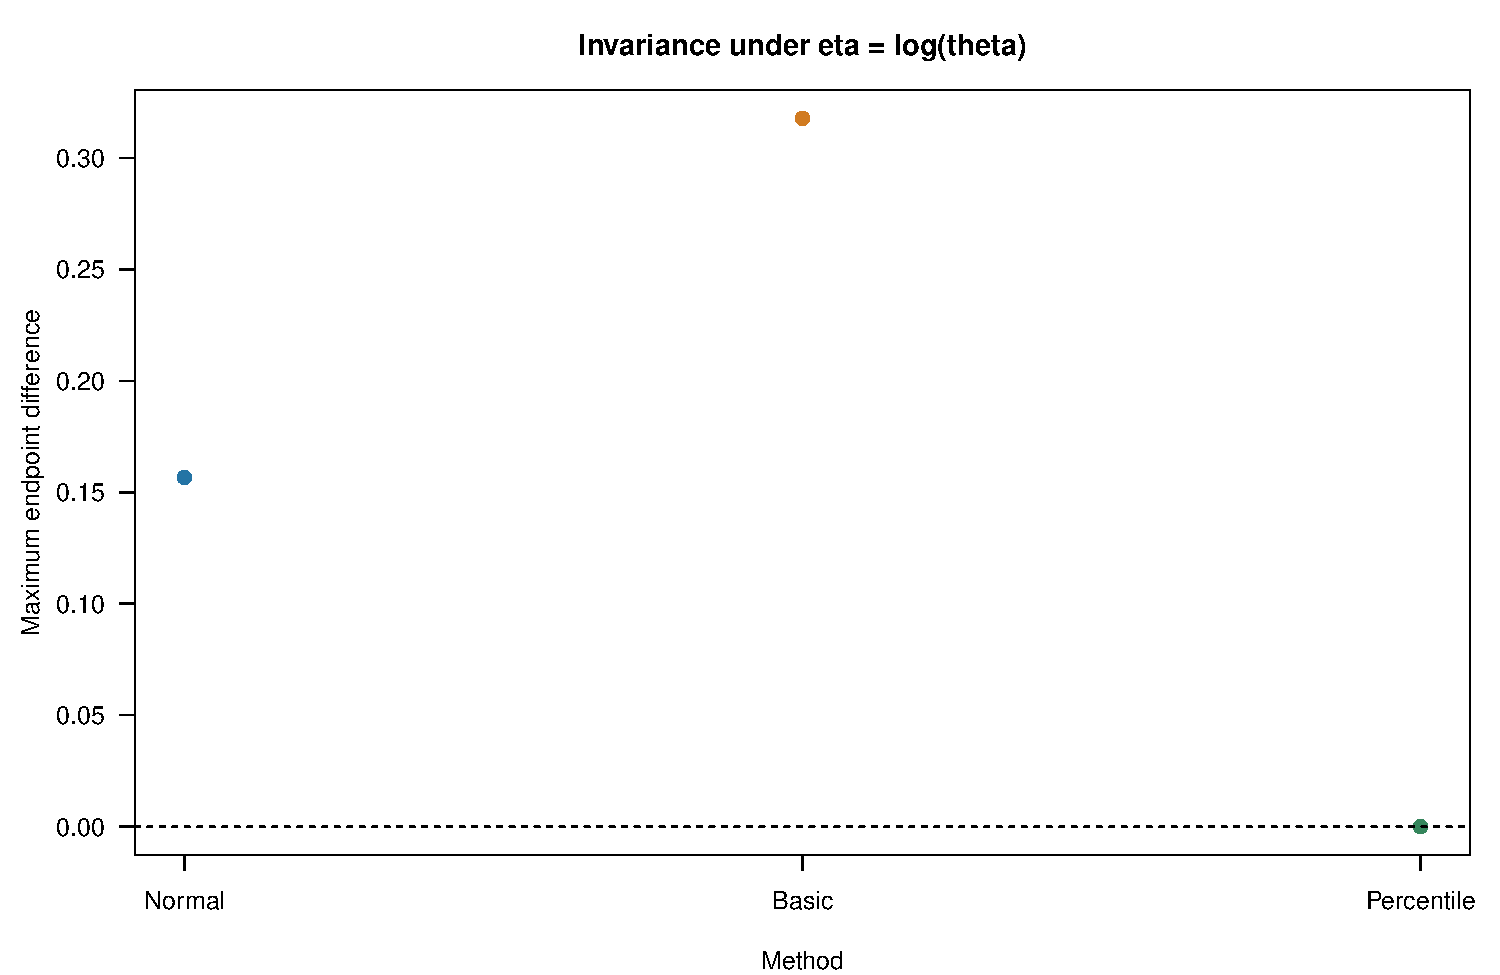
\includegraphics[width=\linewidth,height=4.1cm,keepaspectratio]{../assets/simulate-results/invariance-log-comparison.pdf}
\end{center}
\small Log tăng trên các giá trị dương nên giữ nguyên thứ hạng. Với type~1, lấy log của giá trị ở hạng $\lceil Bp\rceil$ cho đúng phân vị $p$ trên thang log. Vì vậy hai cận Percentile trùng nhau.
\end{frame}
\subsection{Điều kiện áp dụng và giới hạn kết luận}
% Frame 26. Source: Phần 2, 4 và 9. Goal: Giả định và giới hạn tổng quát hóa. Asset: none.
\begin{frame}[label=frame:24]{Điều kiện áp dụng và giới hạn kết luận}
\begin{itemize}
    \item Với mẫu i.i.d., có thể lấy lại từng quan sát. Với dữ liệu phụ thuộc hoặc phân tầng, chọn cách lấy mẫu theo cấu trúc dữ liệu.
    \item Mẫu nhỏ, thống kê không trơn hoặc tham số gần biên có thể làm xấp xỉ Bootstrap kém.
    \item Kết quả coverage chỉ mô tả trung bình mẫu ở hai tổng thể và hai cỡ mẫu đã xét.
\end{itemize}
\end{frame}
\section{Kết luận và giới hạn}
\subsection{Kết luận và khuyến nghị}
% Frame 27. Source: Phần 9. Goal: Tóm tắt kết quả trong phạm vi khảo sát. Asset: none.
\begin{frame}[label=frame:25]{Kết luận và khuyến nghị}
\begin{itemize}
    \item Normal dựa vào sai số chuẩn; Basic phản chiếu phân vị. Kiểm tra hình dạng phân phối, độ chệch và miền tham số trước khi chọn.
    \item Trong mô phỏng, cả ba phương pháp đều dưới $95\%$; cân nhắc độ bao phủ cùng độ dài khoảng.
    \item Khi đổi thang đo, kiểm tra tính bất biến của phương pháp và quy ước phân vị; có thể khảo sát thêm BCa nếu điều kiện phù hợp.
\end{itemize}
\end{frame}
\subsection{Cảm ơn}
% Frame 28. Source: Kết thúc.
\begin{frame}[plain]{Cảm ơn}
    \centering
    \Large Cảm ơn cô và các bạn đã lắng nghe.
\end{frame}
\end{document}
